% Appendix A

\chapter{Experimental Results} % Main appendix title

\label{AppendixA} % For referencing this appendix elsewhere, use \ref{AppendixA}

\section{Document Extraction}

Given below are few scanned images and their corresponding document extractions.

\begin{figure}[th]
	\centering
	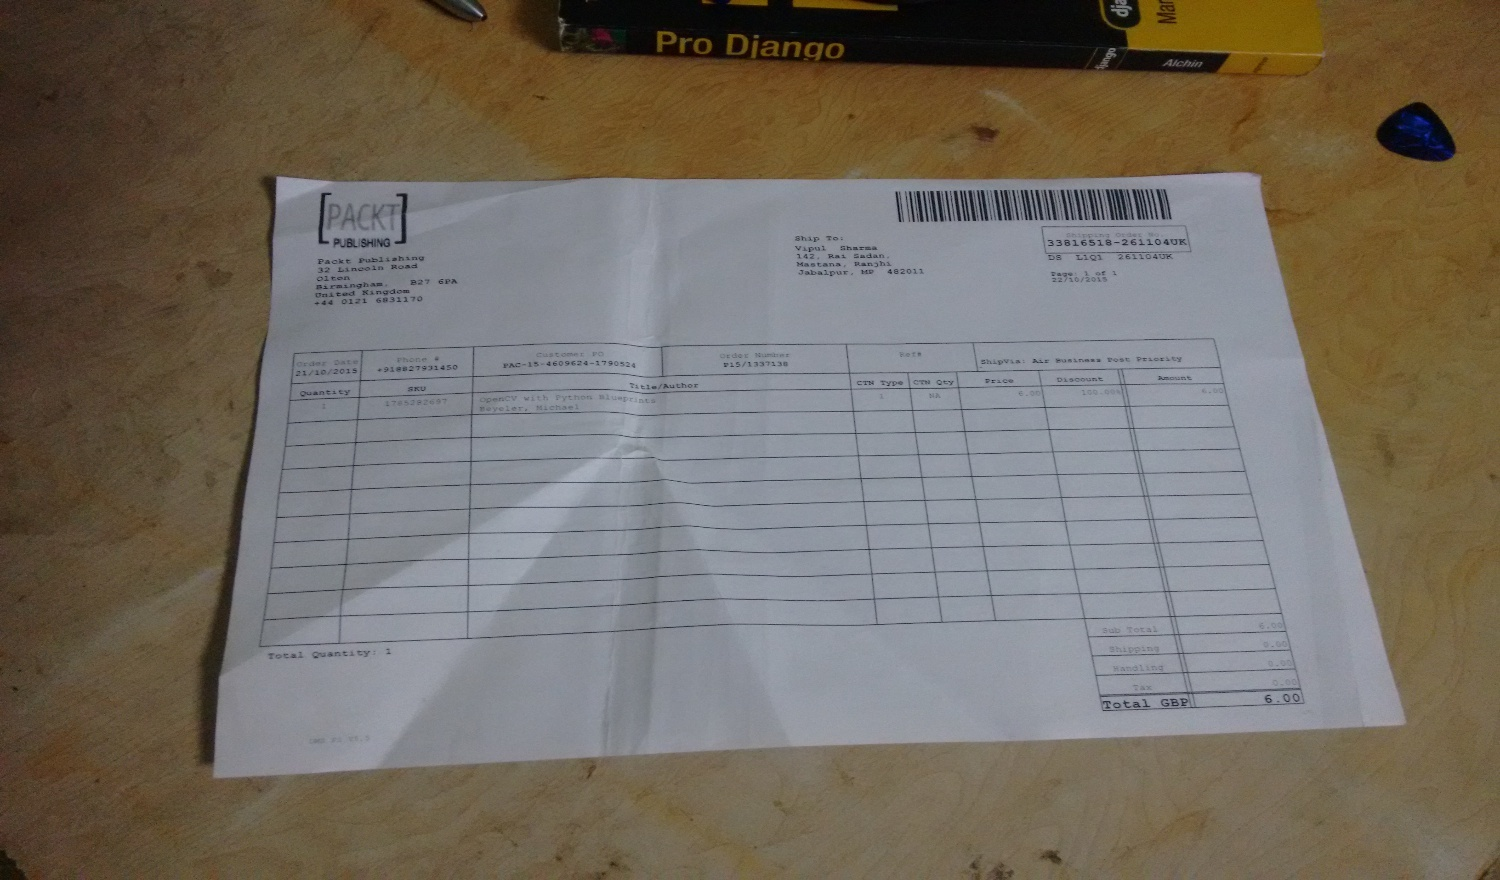
\includegraphics[height=8.8cm ]{Figures/scanned_image2}
	%	\decoRule
	\caption[Scanned Image 2]{Scanned Image 2 (Source : images.google.com).}
	\label{fig:ScannedImage2}
\end{figure}

\begin{figure}[th]
	\centering
	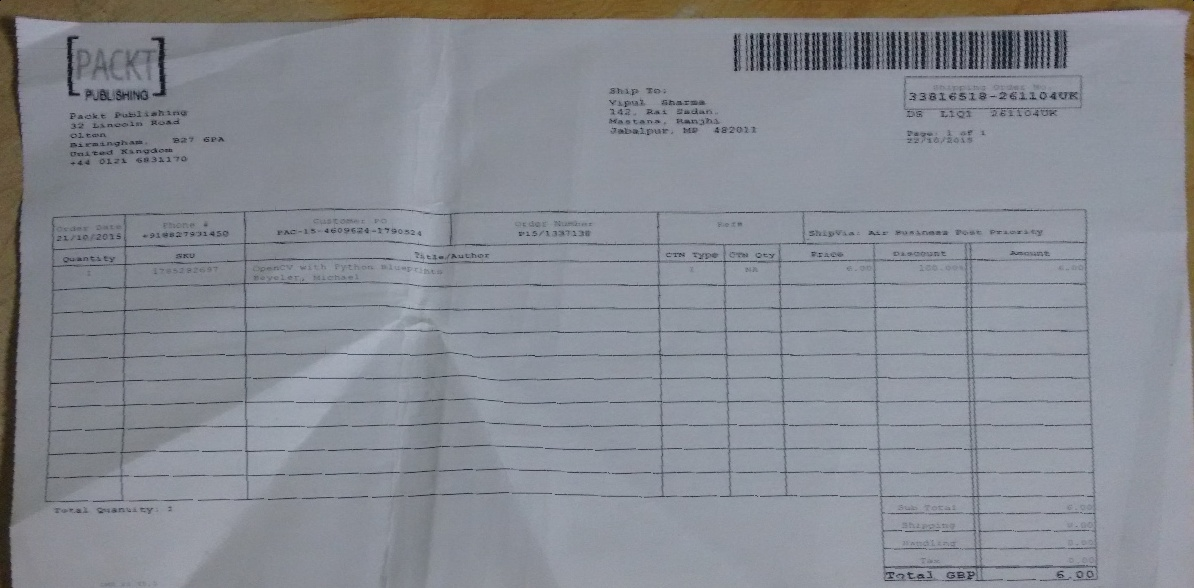
\includegraphics[height=7.5cm ]{Figures/warped_image2}
	%	\decoRule
	\caption[Warped Image 2]{Warped Image 2.}
	\label{fig:WarpedImage2}
\end{figure}

\pagebreak

\begin{figure}[th]
	\centering
	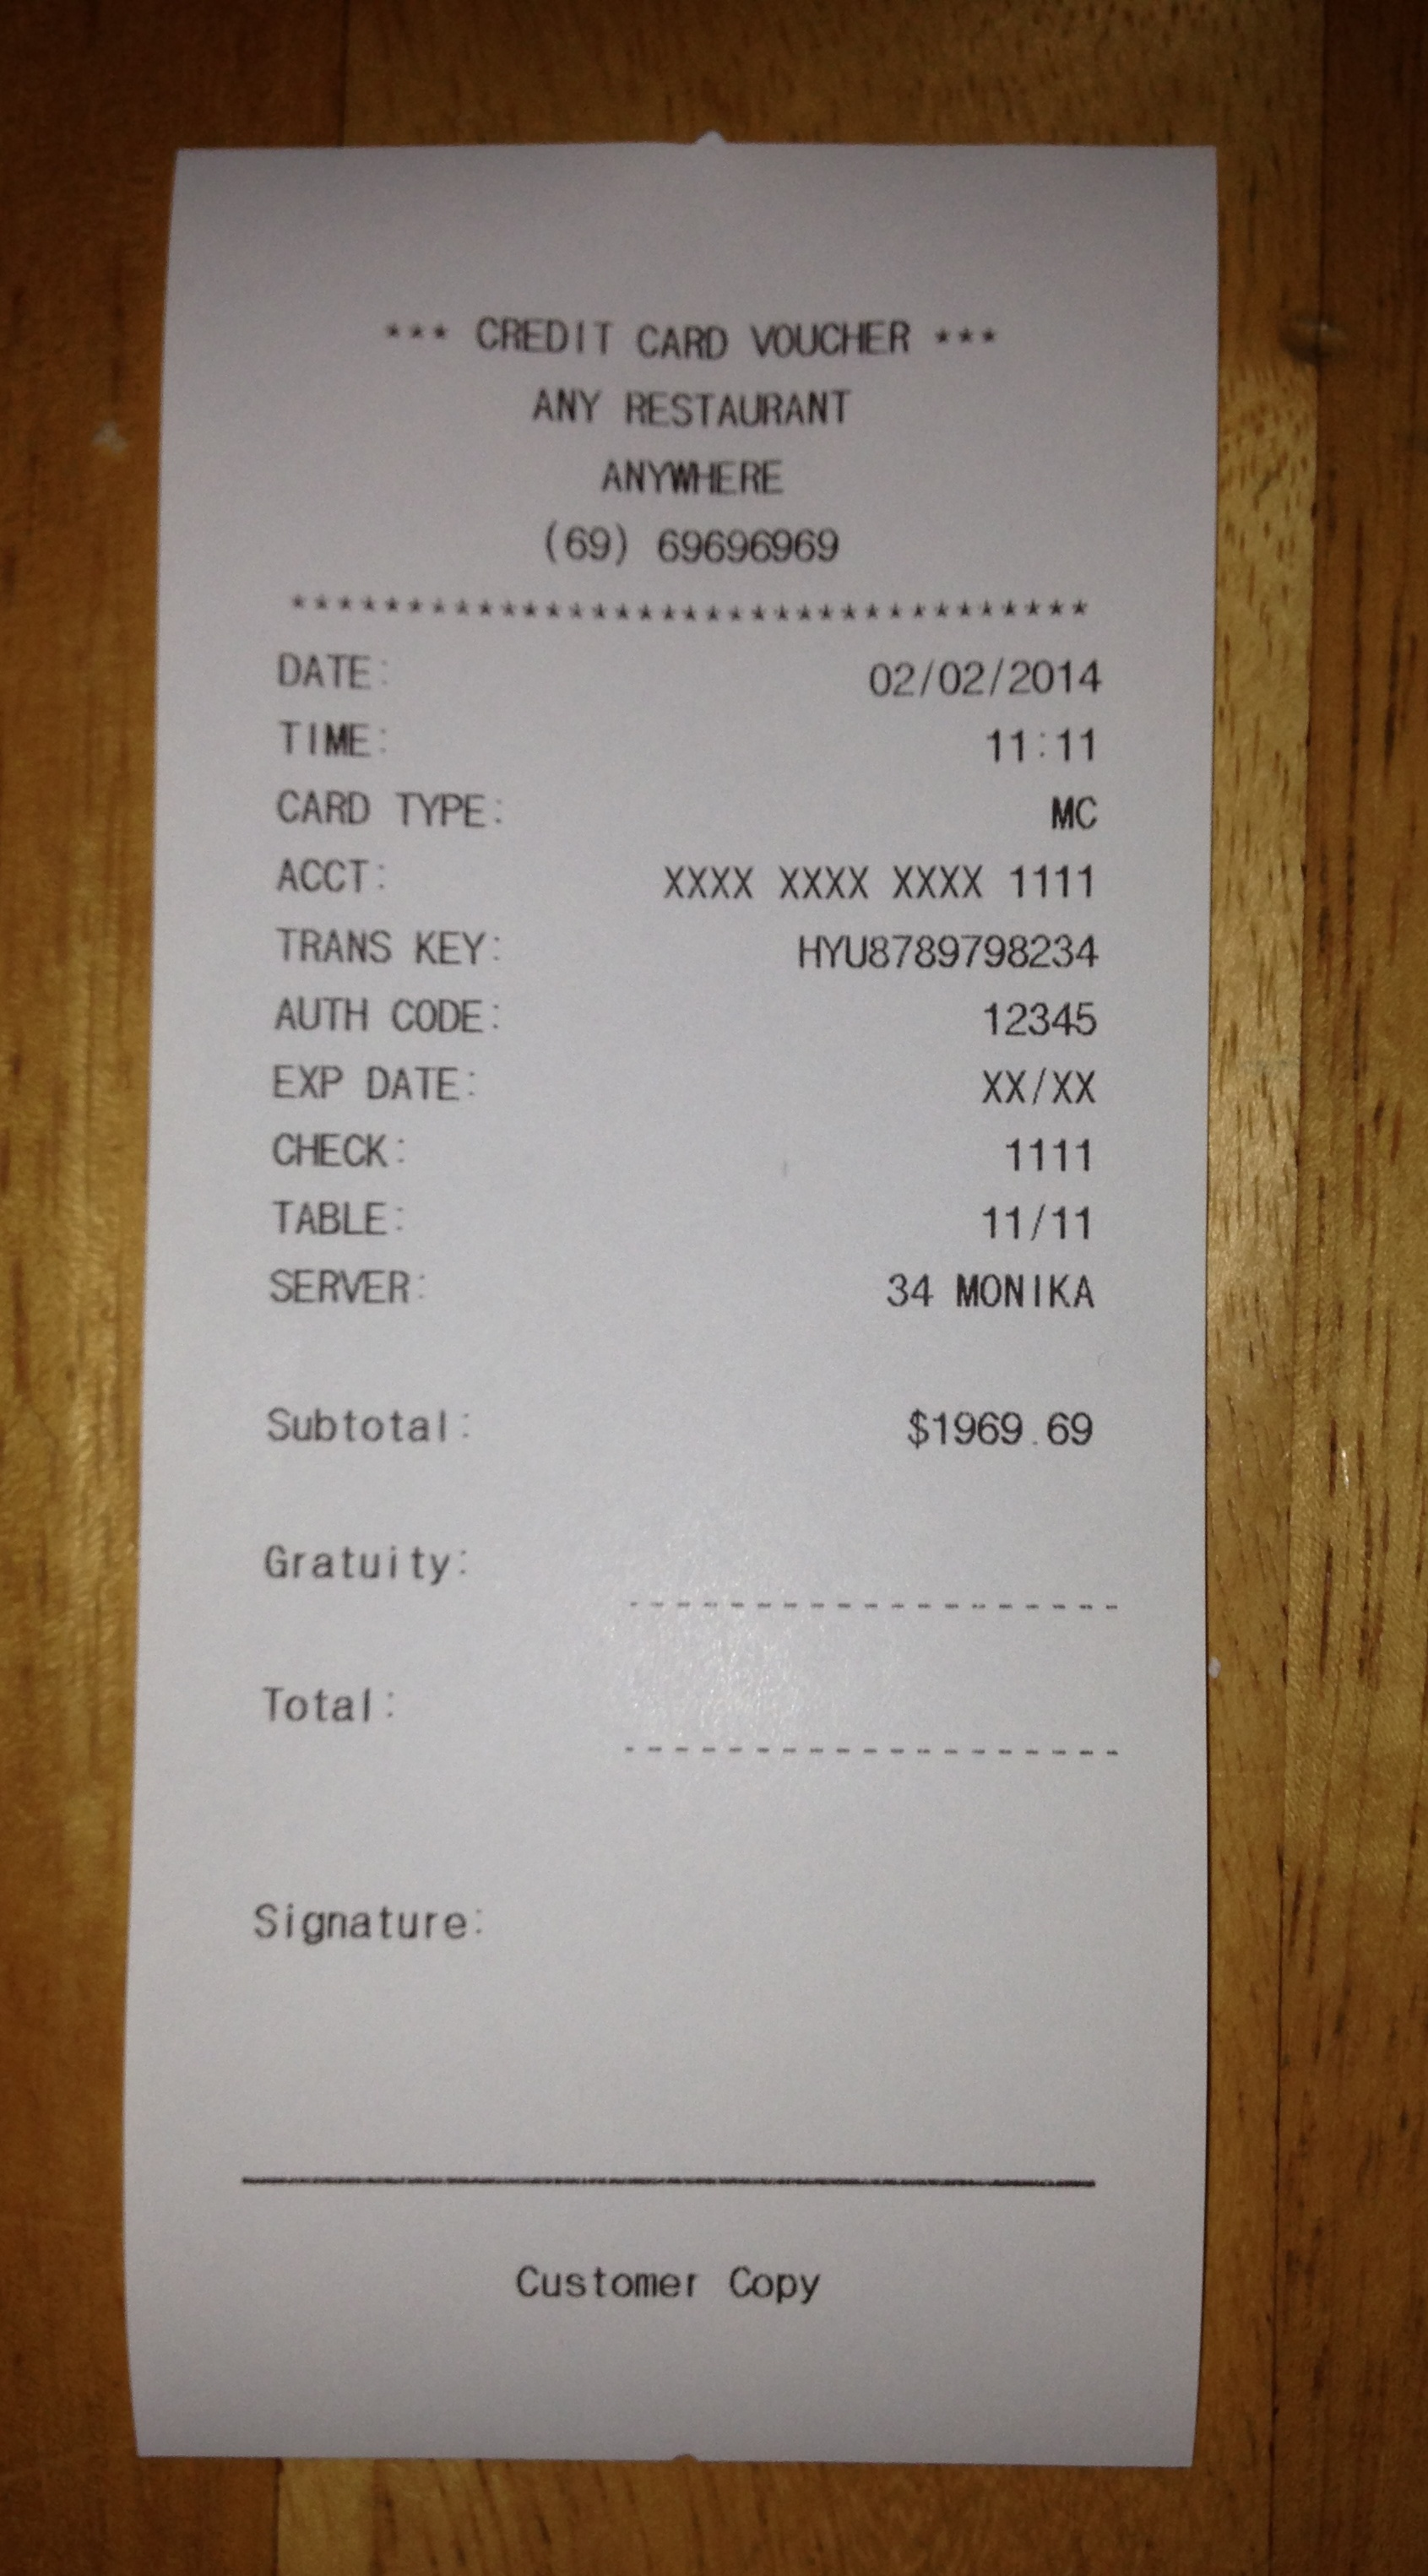
\includegraphics[height=8.5cm ]{Figures/scanned_image3}
	%	\decoRule
	\caption[Scanned Image 3]{Scanned Image 3 (Source : images.google.com).}
	\label{fig:ScannedImage3}
\end{figure}

\begin{figure}[th]
	\centering
	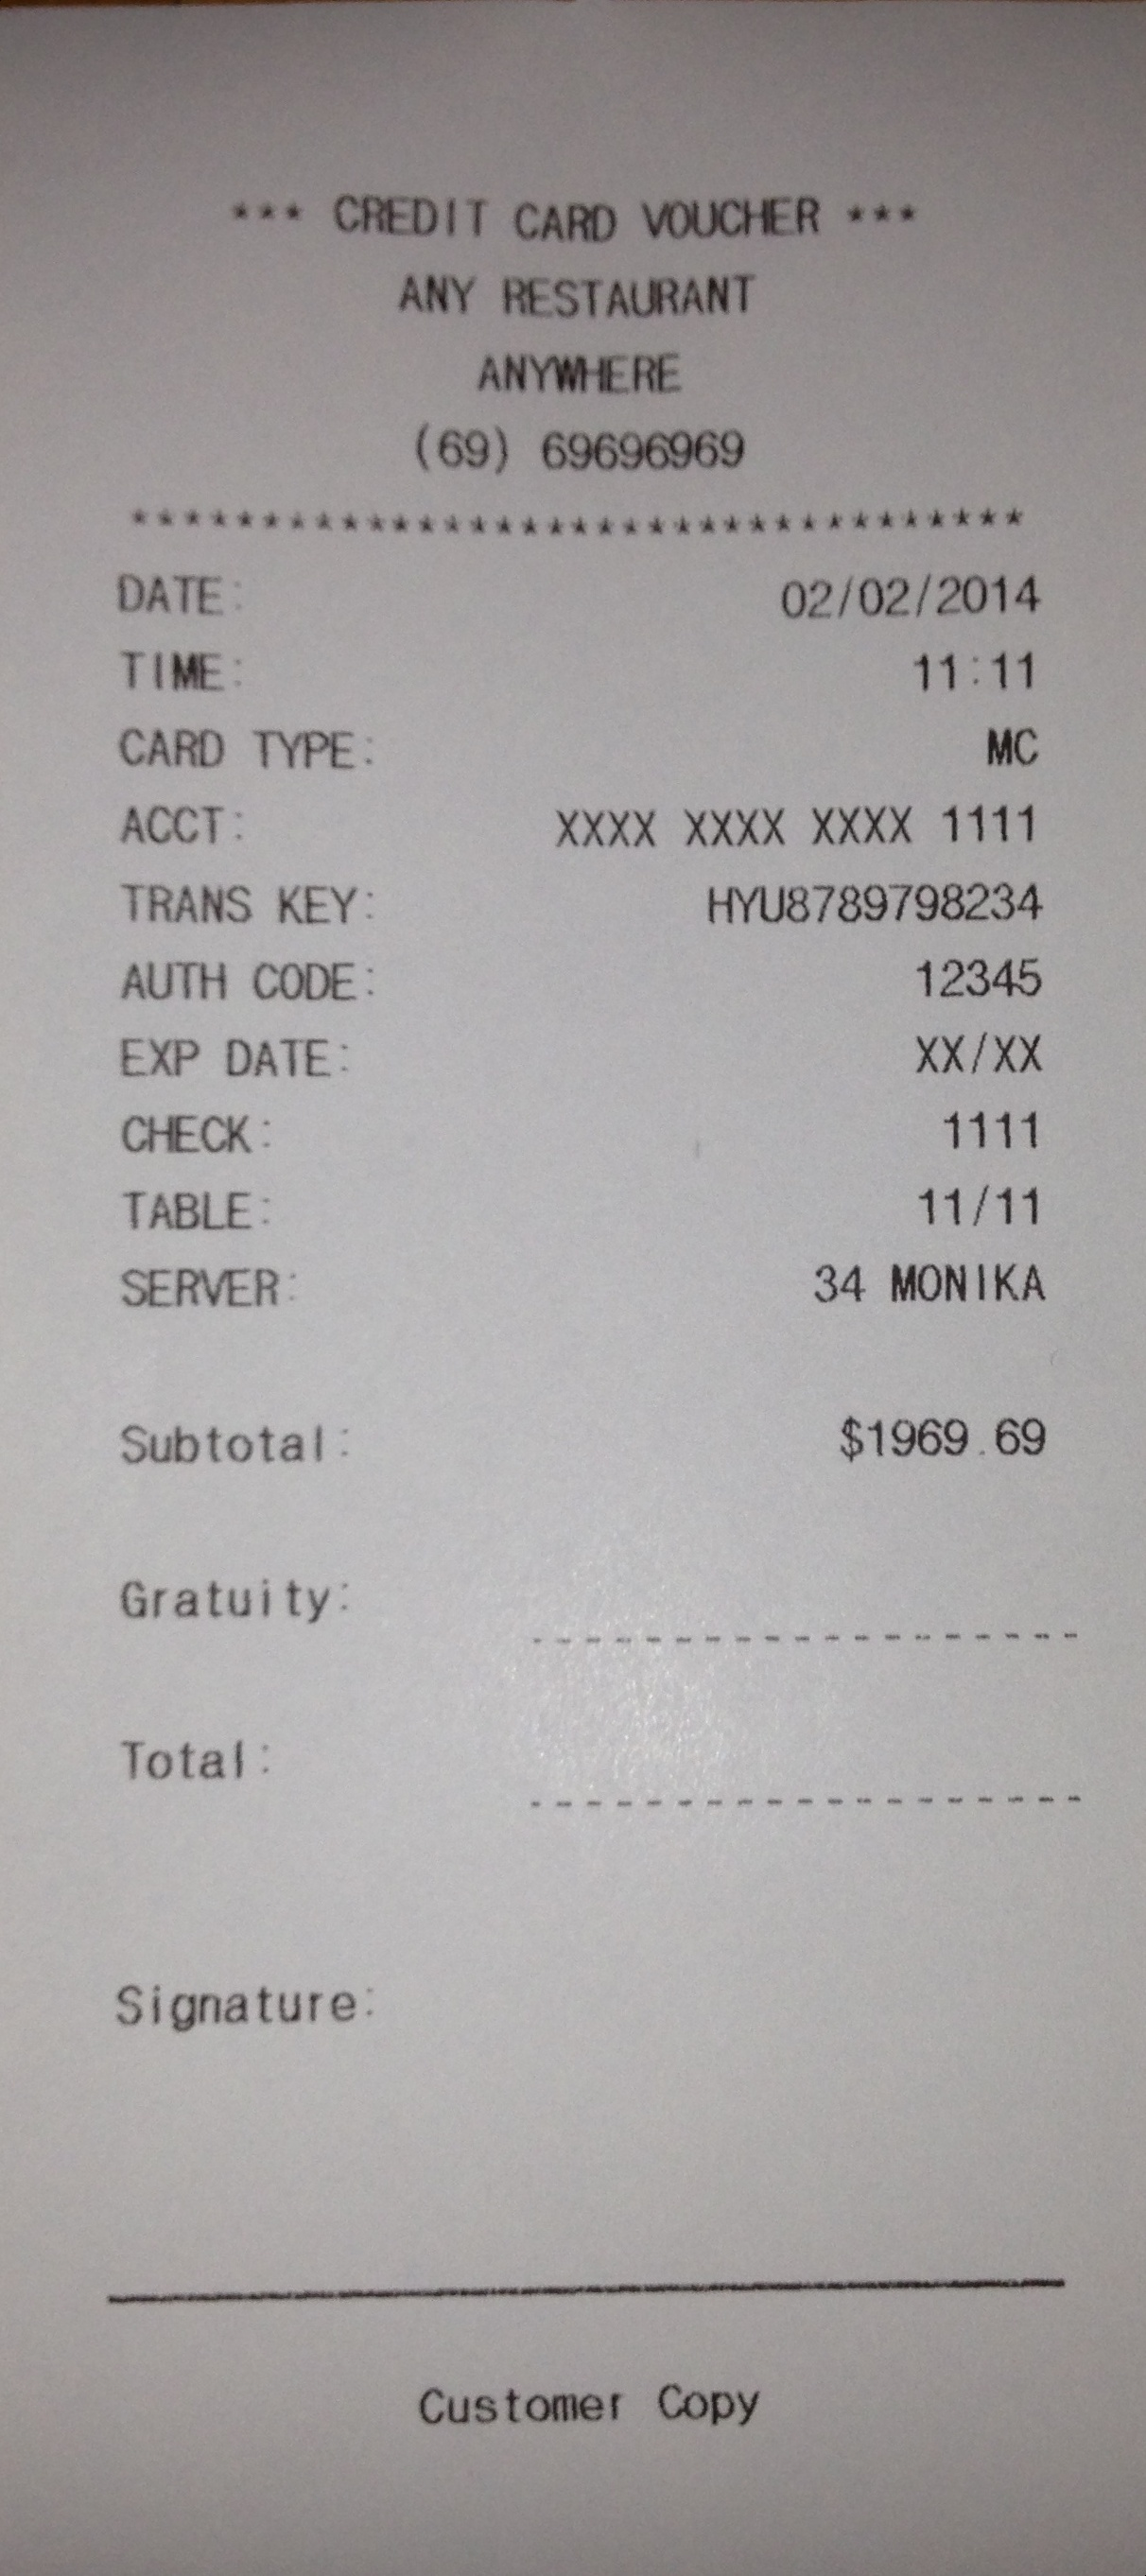
\includegraphics[height=8cm ]{Figures/warped_image3}
	%	\decoRule
	\caption[Warped Image 3]{Warped Image 3.}
	\label{fig:WarpedImage3}
\end{figure}

\pagebreak

\section{Image Registration}

Given below are few reference documents and scanned images and their corresponding image registrations/content extractions.

\begin{figure}[th]
	\centering
	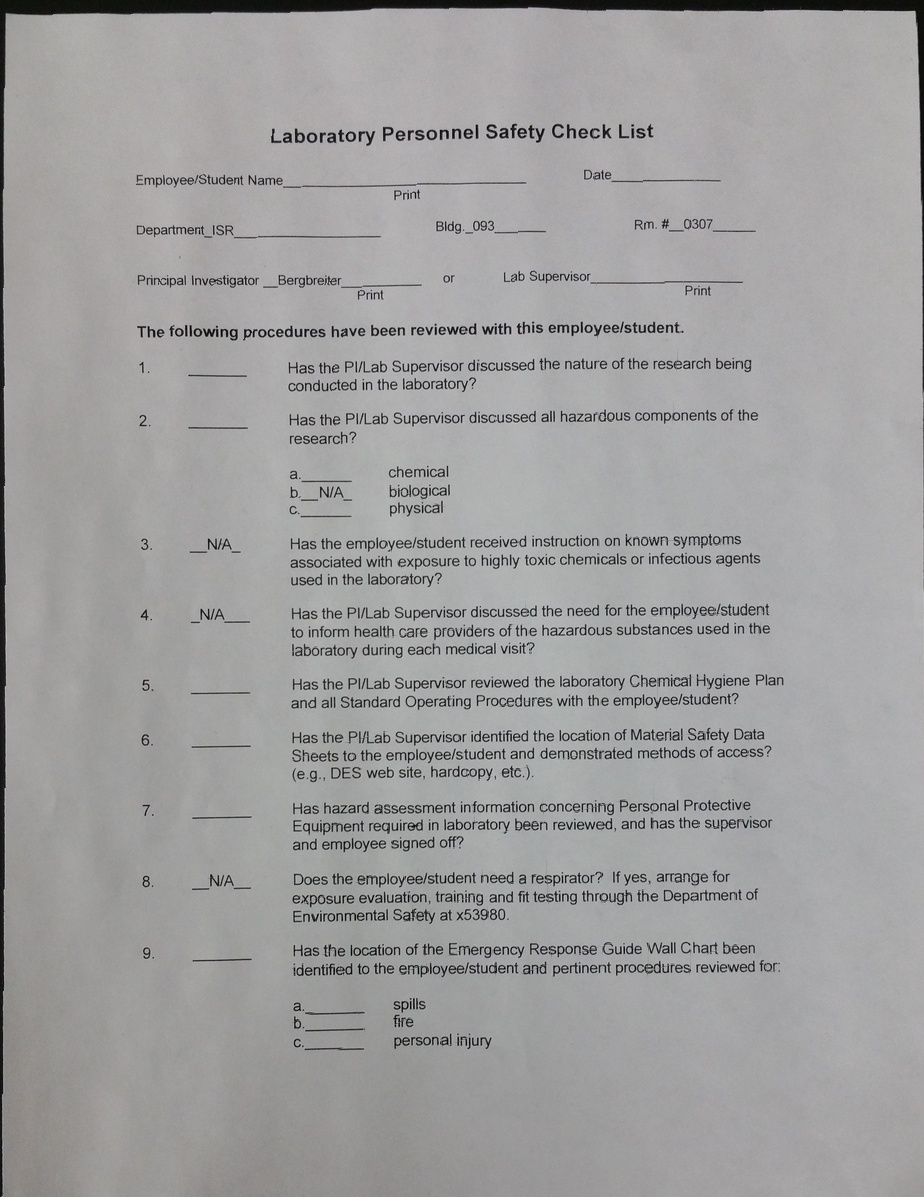
\includegraphics[height=18cm ]{Figures/reference_image2}
	%	\decoRule
	\caption[Reference Image 2]{Reference Image 2.}
	\label{fig:ReferenceImage2}
\end{figure}
\pagebreak
\begin{figure}[th]
	\centering
	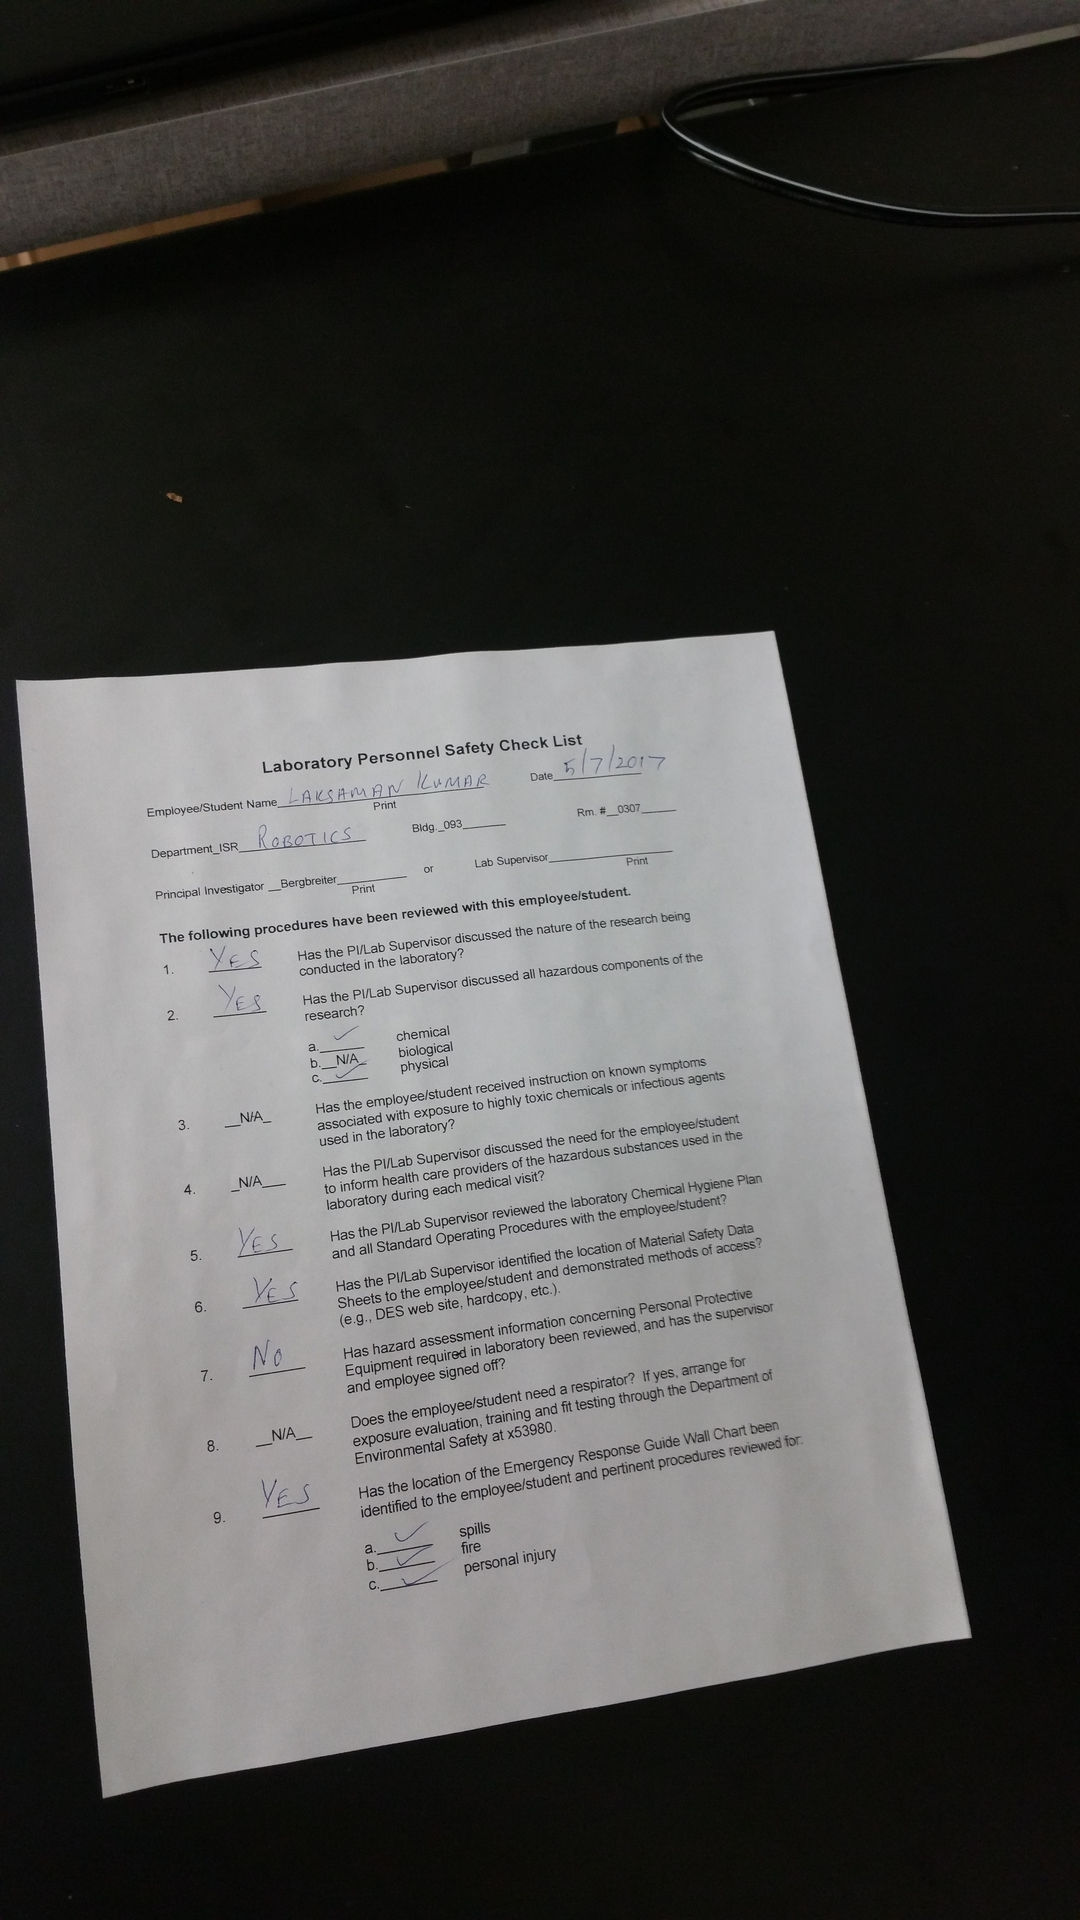
\includegraphics[height=19cm ]{Figures/filled_document1}
	%	\decoRule
	\caption[Filled Document]{Filled Document.}
	\label{fig:FilledDocument}
\end{figure}
\pagebreak
\begin{figure}[th]
	\centering
	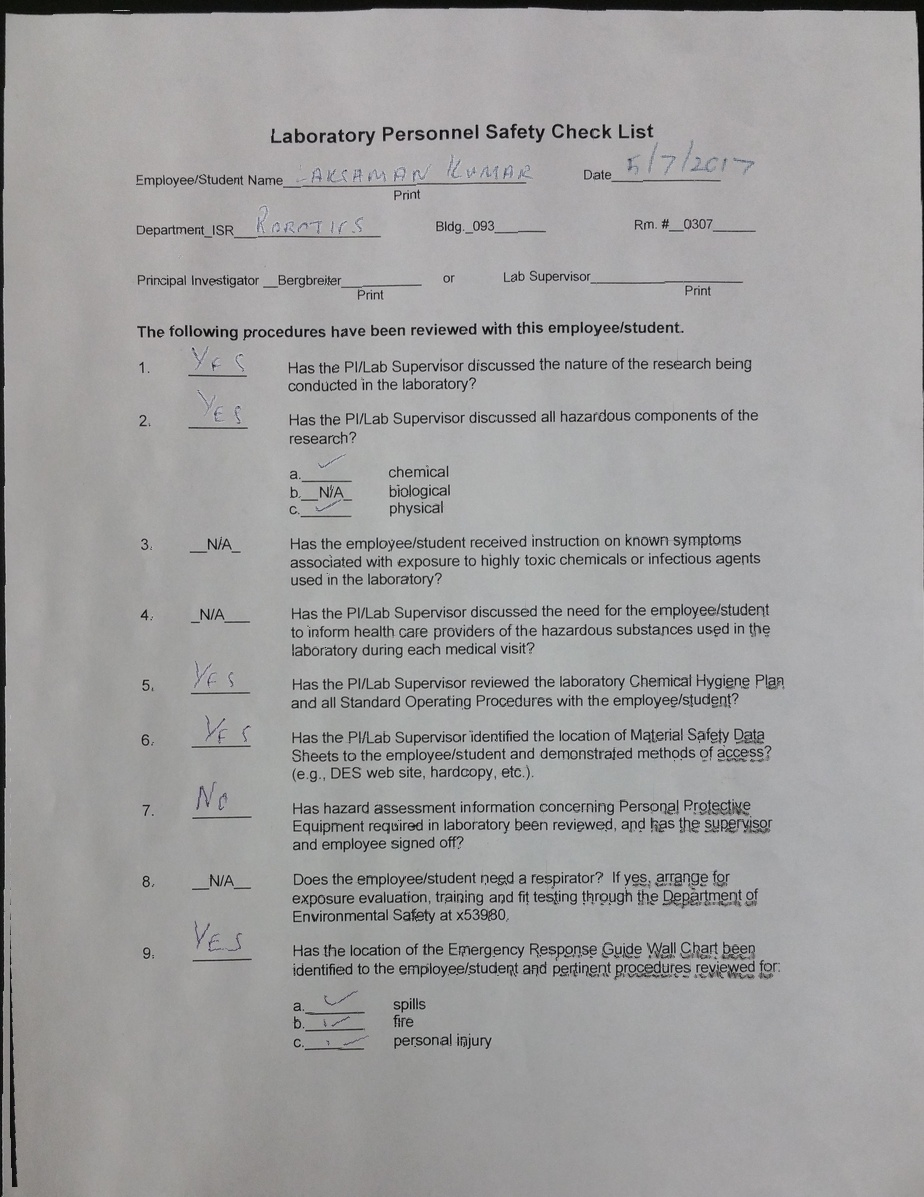
\includegraphics[height=19cm ]{Figures/restored_image2}
	%	\decoRule
	\caption[Restored Image 2]{Restored Image 2.}
	\label{fig:RestoredImage2}
\end{figure}
\pagebreak
\begin{figure}[th]
	\centering
	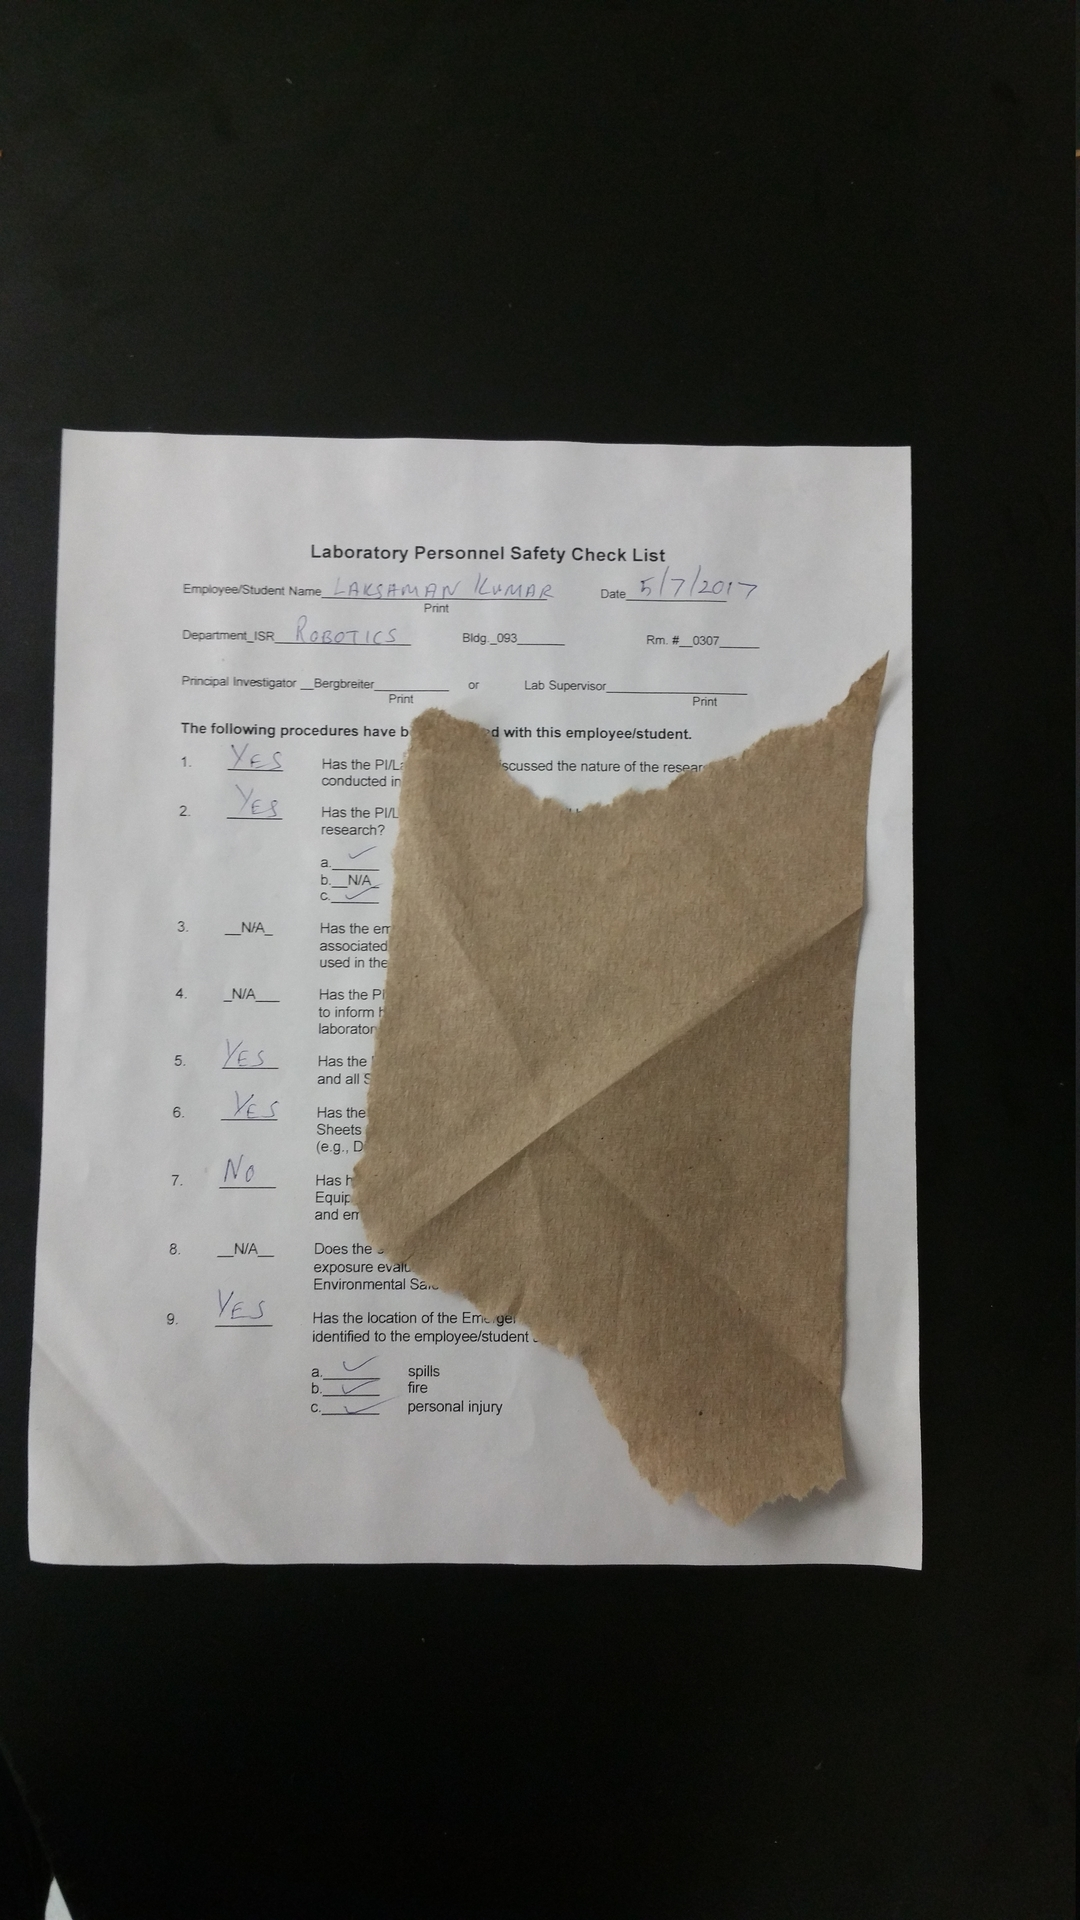
\includegraphics[height=19cm ]{Figures/filled_document2}
	%	\decoRule
	\caption[Filled Document 2]{Filled Document 2.}
	\label{fig:FilledDocument2}
\end{figure}
\pagebreak
\begin{figure}[th]
	\centering
	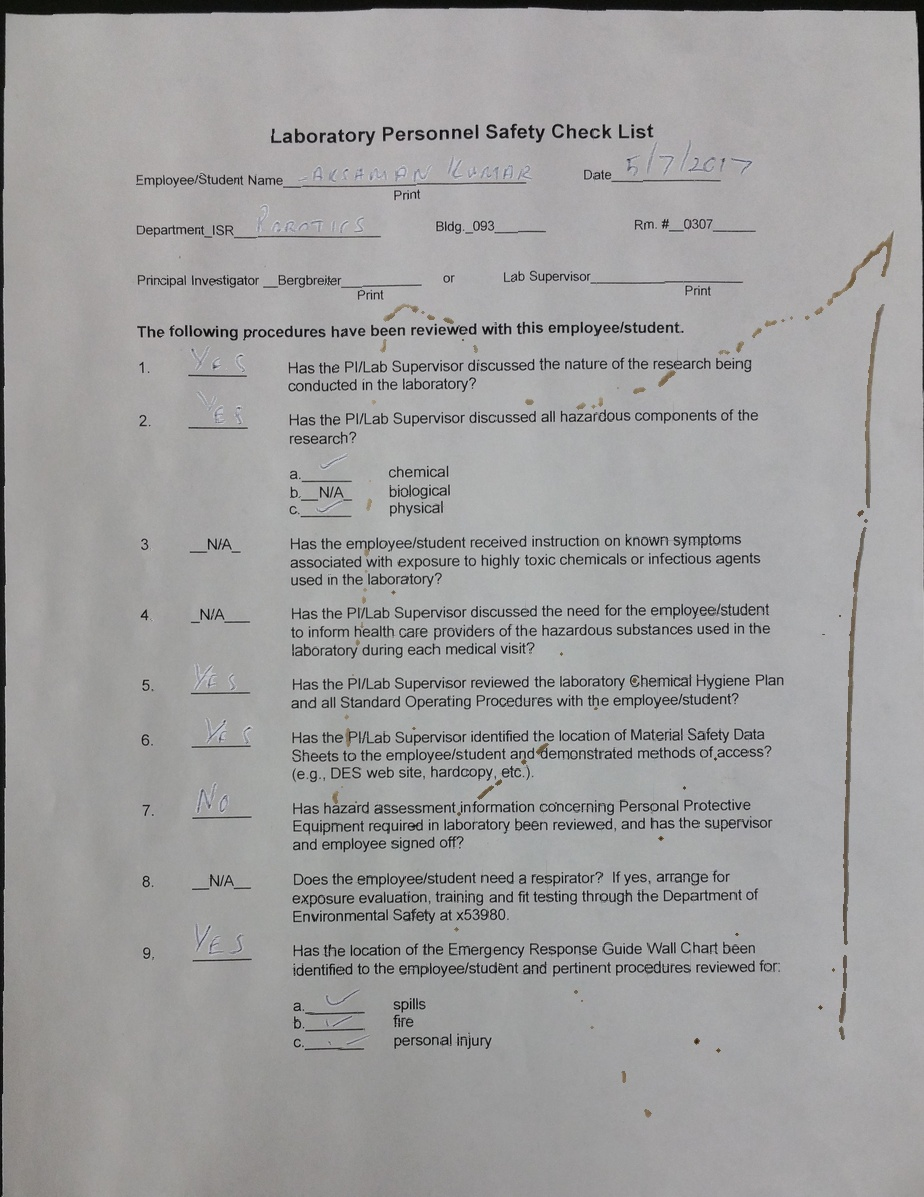
\includegraphics[height=19cm ]{Figures/restored_image3}
	%	\decoRule
	\caption[Restored Image 3]{Restored Image 3.}
	\label{fig:RestoredImage3}
\end{figure}
